\documentclass[12pt]{article}

\usepackage{amsmath}
\usepackage{graphicx}
\usepackage{booktabs}
\usepackage[hidelinks]{hyperref}
\usepackage[numbers]{natbib}
\usepackage{float}
\title{Report 1: Attention Task Validation}

\author{
Team: Chennai Super Kings \\
}

\date{\today}

\begin{document}

\maketitle
\tableofcontents


\section{Introduction}

\subsection{Domain Background}

Selective attention is the cognitive ability to focus on relevant stimuli
while filtering out distractors \citep{treisman1980feature}.
It is fundamental to everyday functioning and is impaired in conditions
such as ADHD and following traumatic brain injury.

The standard laboratory method for measuring selective attention is the
\emph{visual search task}: a participant views a display of objects and
must find a target as quickly and accurately as possible.
Feature Integration Theory predicts that increasing the number of targets
increases attentional load, producing slower reaction times and lower
accuracy \citep{treisman1980feature}.

Laboratory-based assessment, while valid, has practical limitations.
It requires specialised hardware, trained staff, and in-person attendance.
Gamified mobile assessments have been proposed as a scalable alternative,
but must be validated against established lab measures before they can
be trusted \citep{lumsden2016gamification}.

Code is available on \href{https://github.com/jewelj16/Attention-Task-Validation-Data-Analysis}{GitHub}.
% Study Objectives subsection removed as requested.

\subsection{Research Hypotheses}

\subsubsection*{H1 --- Concurrent Validity}
\begin{itemize}
  \item[$H_0$:] There is no correlation between performance on the Game and Lab task ($r = 0$).
  \item[$H_1$:] Performance on the Game task is positively correlated with performance on the Lab task ($r > 0$, one-tailed).
\end{itemize}

\subsubsection*{H2 --- Load Effect}
\begin{itemize}
  \item[$H_0$:] RT and accuracy do not differ between the Single Target and Multiple Target conditions ($\mu_{\text{single}} = \mu_{\text{multiple}}$).
  \item[$H_1$:] The Multiple Target condition results in slower RTs and lower accuracies compared to the Single Target condition, reflecting increased attentional load ($\mu_{\text{multiple}} > \mu_{\text{single}}$ for RT; $\mu_{\text{multiple}} < \mu_{\text{single}}$ for accuracy, one-tailed).
\end{itemize}

\subsubsection*{H3 --- Modality Effect}
\begin{itemize}
  \item[$H_0$:] There is no systematic difference in performance between the Lab and Game interfaces ($\mu_{\text{lab}} = \mu_{\text{game}}$).
  \item[$H_1$:] Performance differs systematically between the Lab and Game interfaces ($\mu_{\text{lab}} \neq \mu_{\text{game}}$, two-tailed).
\end{itemize}

\subsubsection*{H4 --- Level Effect}
\begin{itemize}
  \item[$H_0$:] Performance is stable across game levels, with no linear relationship between level and RT ($r = 0$).
  \item[$H_1$:] RT changes systematically across game levels ($r \neq 0$, two-tailed).
\end{itemize}

\subsubsection*{H5 --- Target Colour Effect}
\begin{itemize}
  \item[$H_0$:] Target colour has no effect on RT or accuracy ($\mu_{\text{red}} = \mu_{\text{other}}$).
  \item[$H_1$:] Red targets result in faster RTs and higher accuracy compared to other colours, consistent with Feature Integration Theory \citep{treisman1980feature} ($\mu_{\text{red}} < \mu_{\text{other}}$ for RT; $\mu_{\text{red}} > \mu_{\text{other}}$ for accuracy, one-tailed).
\end{itemize}

\subsection{Participants}

$N = 37$ participants were randomly assigned to one of two Target Load groups.
To control for practice and fatigue effects, the order of modalities (Lab first or Game first) was counterbalanced within each group.

\begin{table}[h]
\centering
\begin{tabular}{lccc}
\toprule
Group & Condition & $n$ & IDs \\
\midrule
Group A & Single Target & 21 & 1--21 \\
Group B & Multiple Target & 16 & 22--37 \\
\bottomrule
\end{tabular}
\caption{Participant allocation}
\end{table}

\section{Methods}

\subsection{Independent and Dependent Variables}

The experiment used a 2 $\times$ 2 Mixed Factorial Design with the following variables:

\textbf{1. Independent Variables (IVs)}
\begin{itemize}
  \item \textbf{Target Load:} (Between-Subjects) Participants were assigned to either \textit{Single Target} (one object to find) or \textit{Multiple Target} (several objects to find at once).
  \item \textbf{Modality:} (Within-Subjects) Every participant played the \textit{Game} on a smartphone and did the \textit{Lab} task on a computer.
\end{itemize}

\textbf{2. Dependent Variables (DVs)}
\begin{itemize}
  \item \textbf{Reaction Time (RT):} The time in seconds it takes from when the target appears to when the participant first clicks or taps it.
  \item \textbf{Accuracy:} The proportion (0 to 1) of correct clicks or taps out of everything the participant did.
\end{itemize}

\subsection{Relevant Data Columns}
The dataset combines lab and game records. Key columns used throughout the notebook are summarized succinctly here: \texttt{participant} (subject ID), \texttt{target\_load} (Single / Multiple), \texttt{modality} (lab / game), \texttt{trial\_num}/\texttt{Level} (trial or level index), \texttt{RT} (reaction time in seconds; lab: computed from mouse timestamps; game: InitialResponseTime(ms)/1000), and \texttt{accuracy} (proportion correct). The lab-only field \texttt{target\_col} is used for colour-related analyses.

\subsection{Reaction Time}

Reaction time (RT) was computed as:

\[
RT = mouse.time[0] - (square.started - trial.started)
\]

For game files:

\[
RT = \frac{InitialResponseTime(ms)}{1000}
\]

\subsection{Accuracy}

\begin{itemize}
\item \textbf{Single target:} Correct if \texttt{target} appears in \texttt{mouse.clicked\_name}.
\item \textbf{Multiple targets:} Correct objects are \texttt{target\_0} to \texttt{target\_4}.
Accuracy = correct selections divided by 5.
\end{itemize}

For game files:

\[
Accuracy = \frac{SuccessRate(\%)}{100}
\]

\subsection{Data Cleaning}

\begin{enumerate}
\item Remove non-trial rows where \texttt{trials.thisN} is missing.
\item Exclude RT $<0.1$ s or $>30$ s.
\item Clip accuracy to the range $[0,1]$.
\end{enumerate}


\section{Results}
\subsection{Descriptive Statistics}

\begin{table}[h]
\centering
\resizebox{\textwidth}{!}{
\begin{tabular}{llccccccccc}
\toprule
 & & & \multicolumn{5}{c}{RT (s)} & \multicolumn{3}{c}{Accuracy} \\
\cmidrule(lr){4-8}\cmidrule(lr){9-11}
Target Load & Modality & $N$ & $M$ & $SD$ & $Med$ & $Min$ & $Max$ & $M$ & $SD$ & $Med$ \\
\midrule
Multiple & Game & 16 & 1.856 & 0.507 & 1.719 & 1.136 & 3.120 & 0.964 & 0.025 & 0.963 \\
         & Lab  & 16 & 1.505 & 0.268 & 1.428 & 1.186 & 2.023 & 0.951 & 0.135 & 0.993 \\
Single   & Game & 21 & 3.104 & 0.625 & 2.923 & 2.258 & 4.683 & 0.983 & 0.028 & 1.000 \\
         & Lab  & 21 & 1.495 & 0.225 & 1.471 & 1.093 & 2.223 & 1.000 & 0.000 & 1.000 \\
\bottomrule
\end{tabular}
}
\caption{Descriptive statistics}
\end{table}
\subsection{Figures}

\begin{figure}[H]
\centering
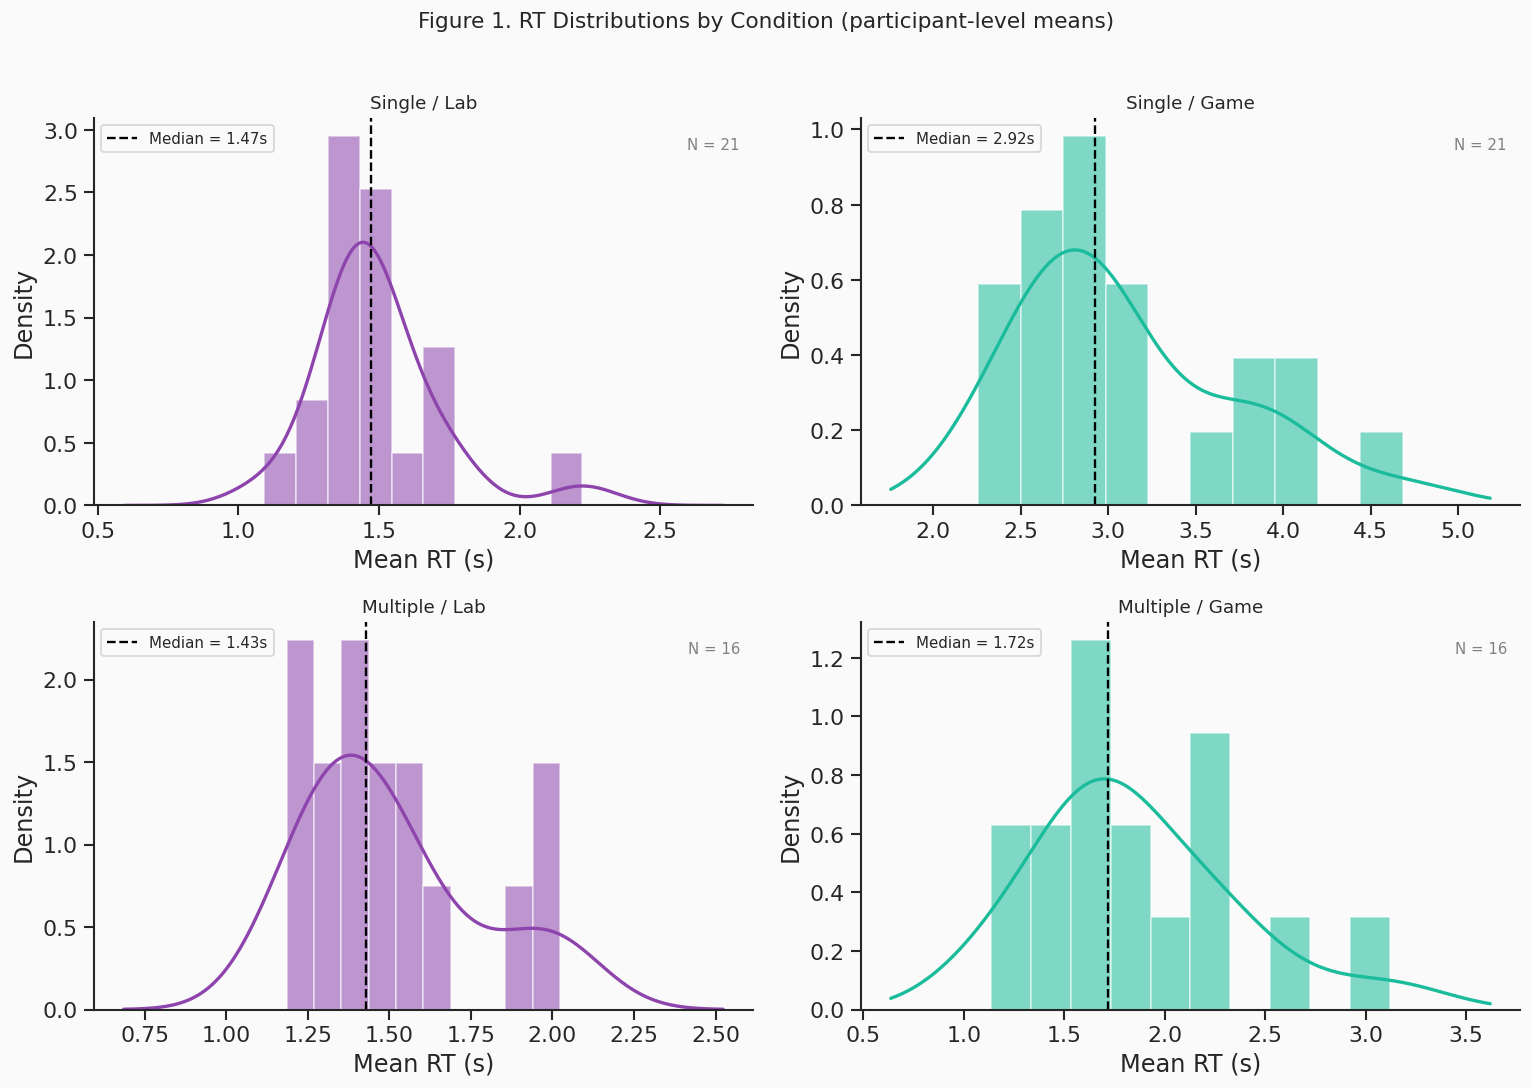
\includegraphics[width=0.7\linewidth]{rt_dist.png}
\caption{Reaction Time Distribution}
\end{figure}

\begin{figure}[H]
\centering
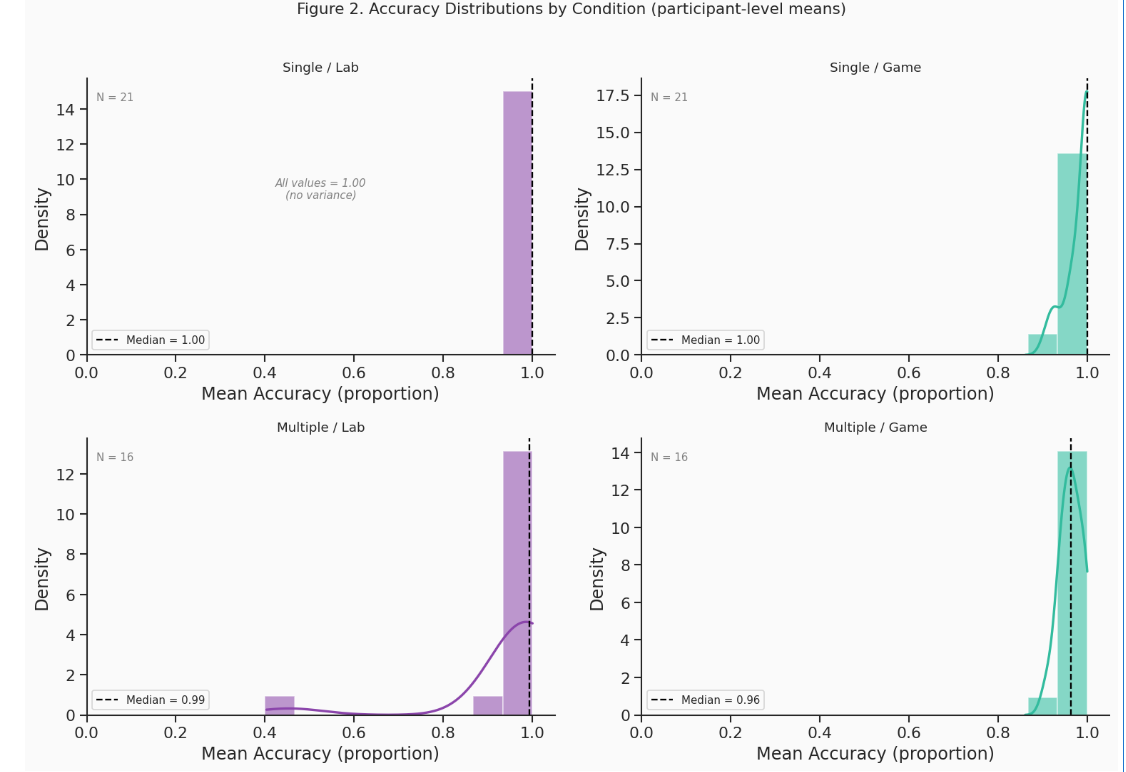
\includegraphics[width=0.7\linewidth]{acc_dist.png}
\caption{Accuracy Distribution}
\end{figure}

\begin{figure}[H]
\centering
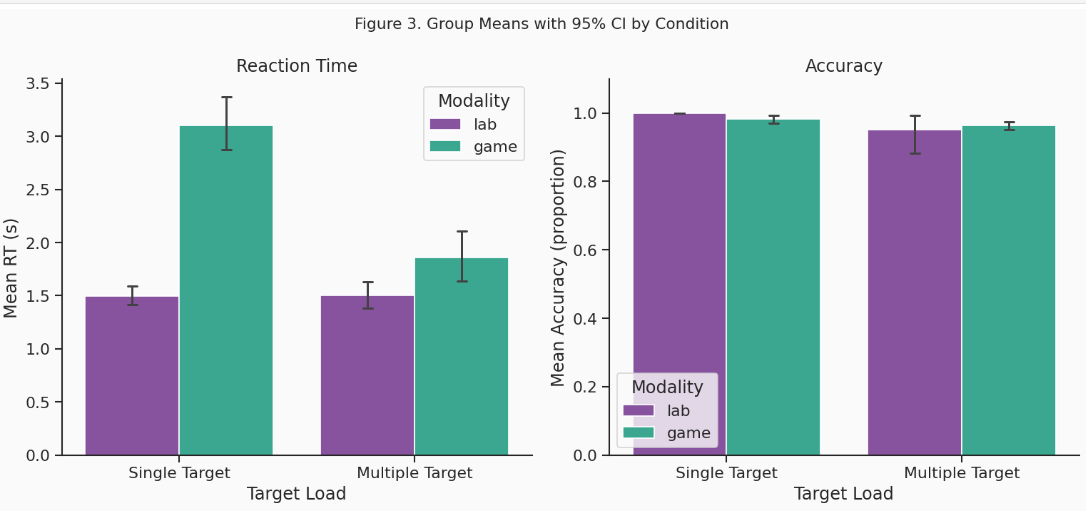
\includegraphics[width=0.7\linewidth]{groups_dist.png}
\caption{Group Distribution}
\end{figure}

\begin{figure}[H]
\centering
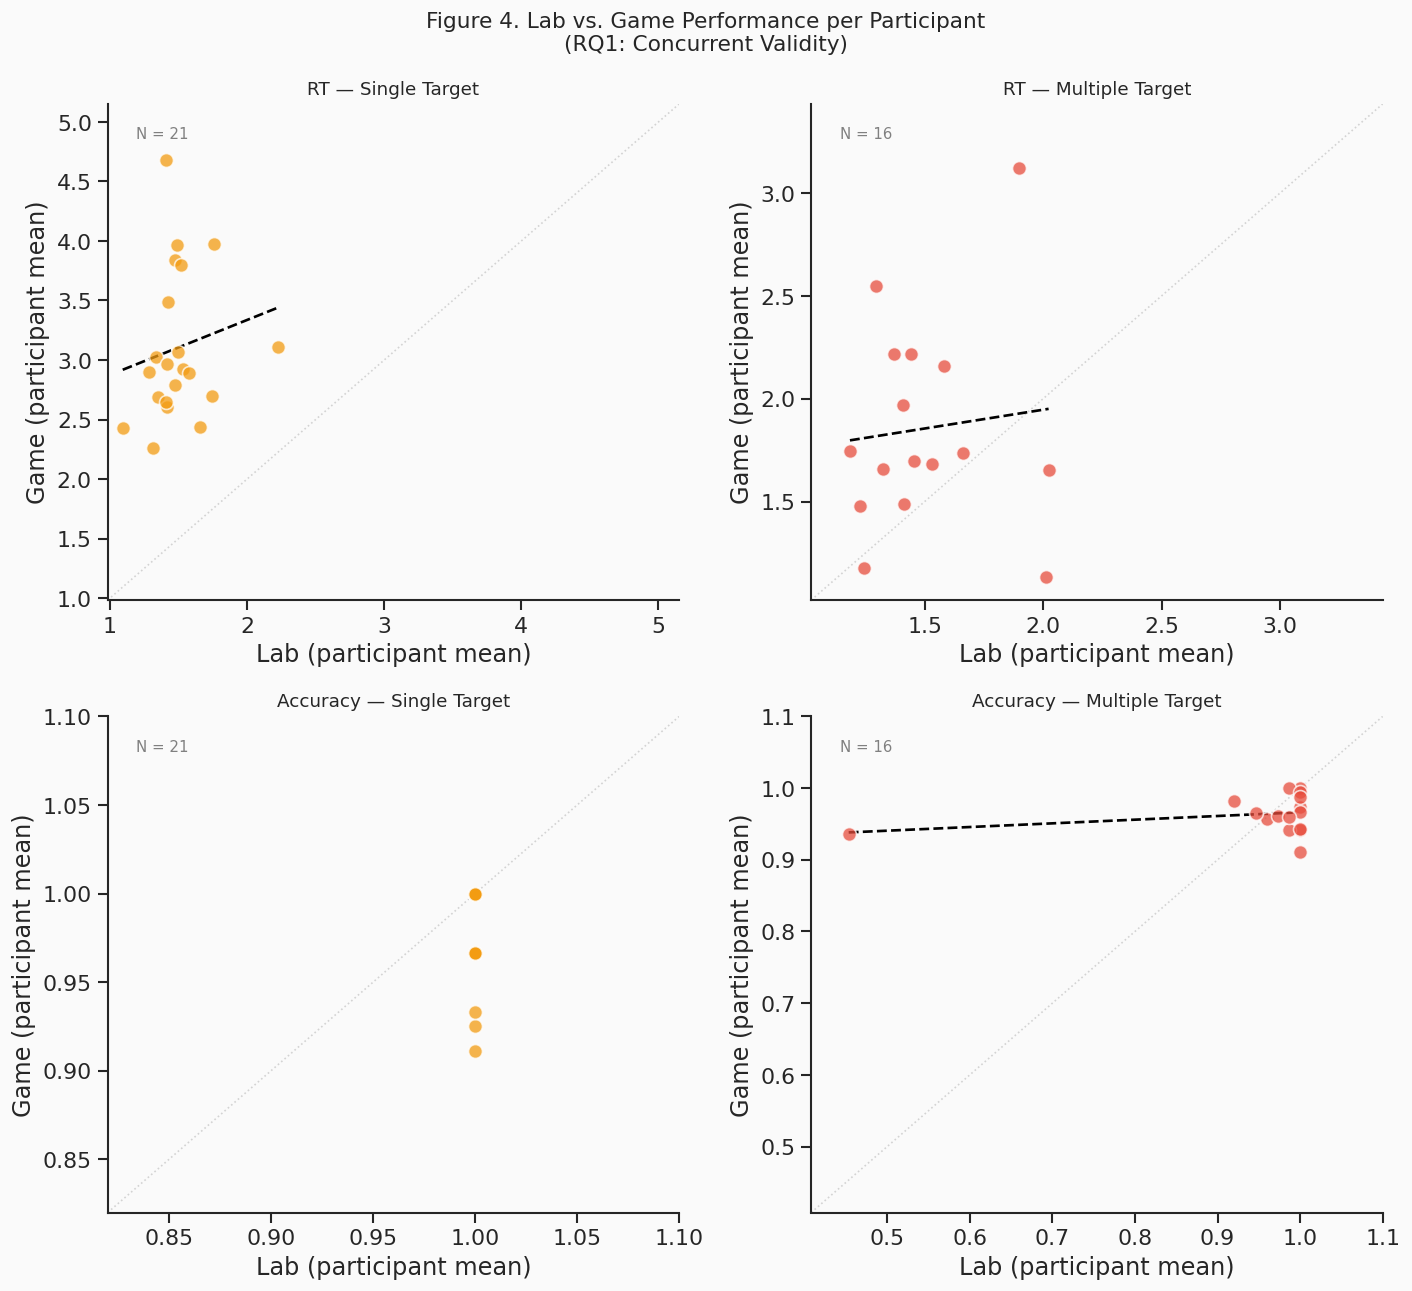
\includegraphics[width=0.7\linewidth]{lab_vs_game.png}
\caption{Lab vs Game Performance}
\end{figure}

\begin{figure}[H]
\centering
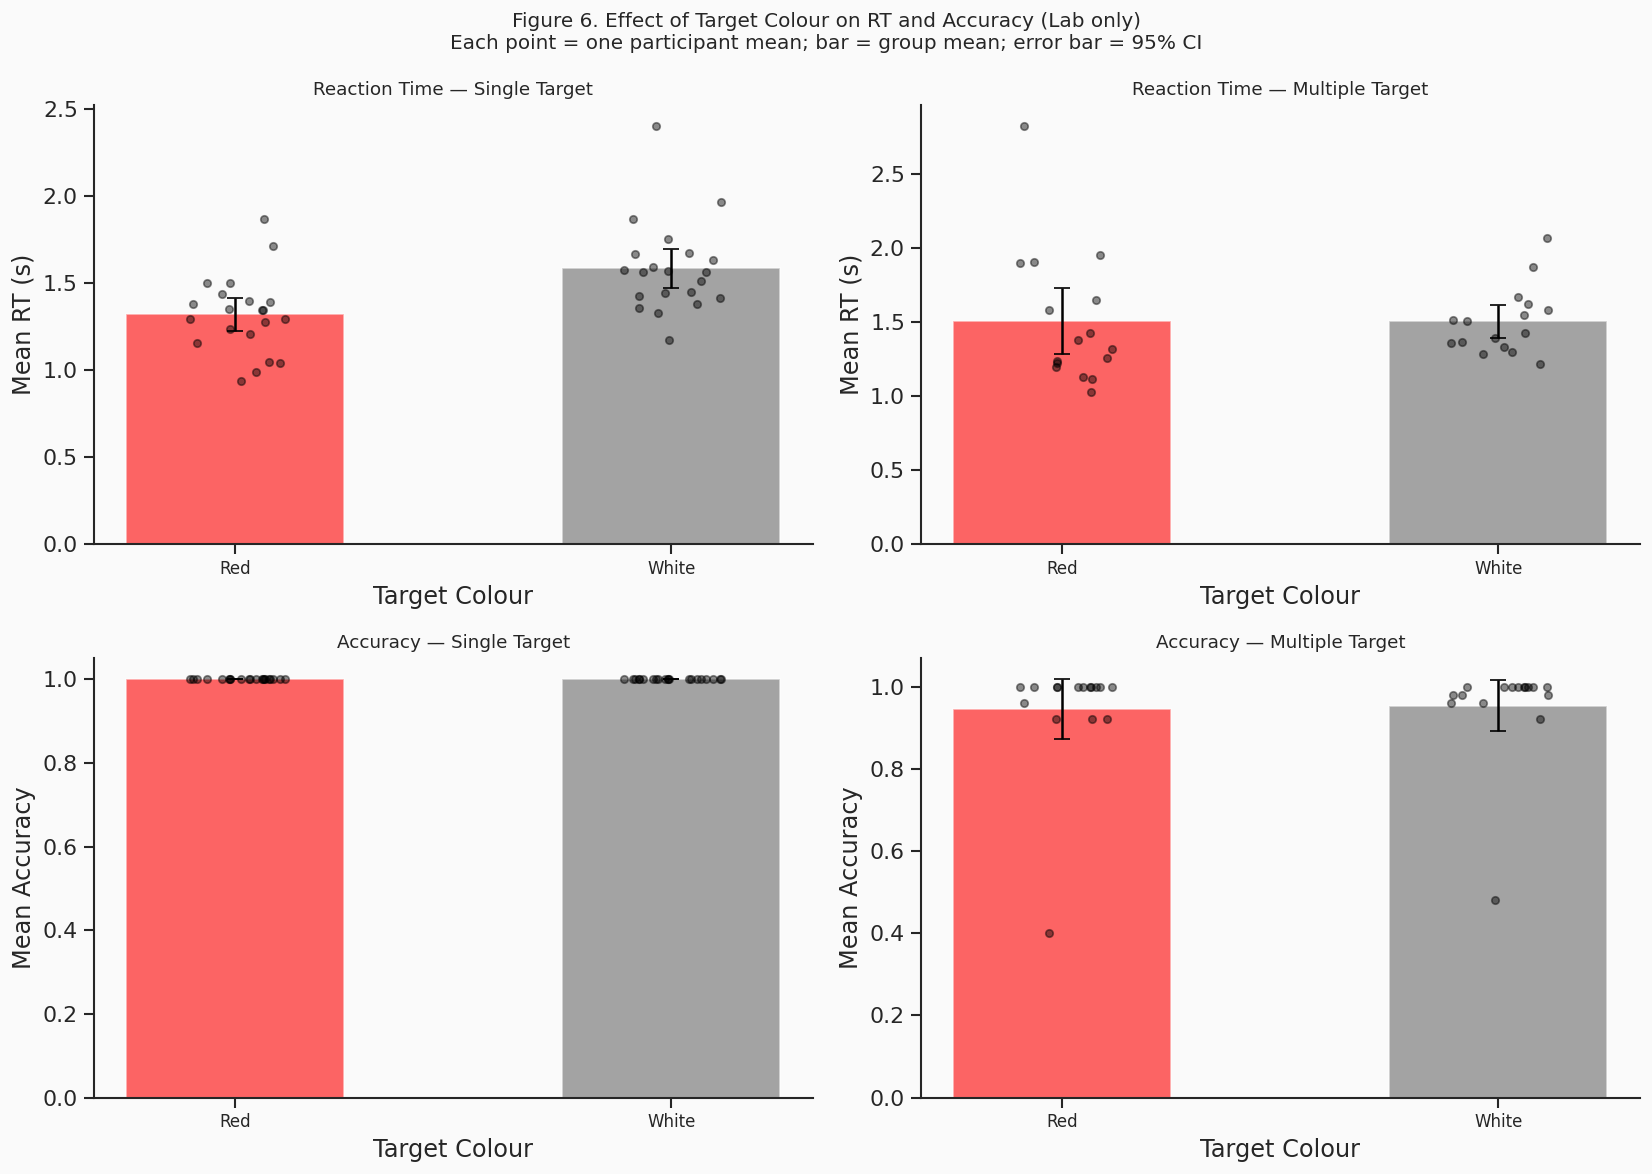
\includegraphics[width=0.7\linewidth]{image.png}
\caption{Effect of Target Colour}
\end{figure}

\section{Future Work}

Future work will entail a comprehensive statistical evaluation of the data to test the research hypotheses, including:

\begin{itemize}
\item \textbf{Correlation Analysis (Concurrent Validity):} Pearson's $r$ or Spearman's $\rho$ to test the relationship between Game and Lab performance across Target Load groups.
\item \textbf{Mixed ANOVA (2 $\times$ 2):} To evaluate the main effects of Modality (Lab vs. Game) and Target Load (Single vs. Multiple), as well as their interaction.
\item \textbf{Paired Samples t-tests (Modality Effect):} Follow-up tests within each group comparing Lab and Game scores for the same participants.
\item \textbf{Independent Samples t-tests (Load Effect):} Follow-up tests within each modality comparing the Single Target group against the Multiple Target group.
\item \textbf{Level Effect Tracking:} Linear regression or correlation examining RT changes across sequential game levels to identify learning or fatigue trends.
\end{itemize}

\section{Member Contributions}

The successful completion of this project was a collaborative effort. The specific contributions of each team member are outlined below:

\begin{itemize}
\item \textbf{Jewel Joseph (2025201047):} Data Summary, Visualizations, and Report drafting
\item \textbf{Gokul C (2025201042):} Visualizations and Exploratory Analysis
\item \textbf{Giridharan P (2025201030):} Visualizations, Literature Research, and Report assistance
\end{itemize}

\bibliographystyle{apalike}

\begin{thebibliography}{2}

\bibitem{lumsden2016gamification}
Lumsden et al. (2016).
Gamification of cognitive assessment and training: A systematic review of applications and efficacy.
\textit{JMIR Serious Games}.

\bibitem{treisman1980feature}
Anne M. Treisman, Garry Gelade (1980).
A feature-integration theory of attention.
\textit{Cognitive Psychology}, Volume 12, Issue 1.



\end{thebibliography}

\end{document}



